
%% bare_conf.tex
%% V1.3
%% 2007/01/11
%% by Michael Shell
%% See:
%% http://www.michaelshell.org/
%% for current contact information.
%%
%% This is a skeleton file demonstrating the use of IEEEtran.cls
%% (requires IEEEtran.cls version 1.7 or later) with an IEEE conference paper.
%%
%% Support sites:
%% http://www.michaelshell.org/tex/ieeetran/
%% http://www.ctan.org/tex-archive/macros/latex/contrib/IEEEtran/
%% and
%% http://www.ieee.org/

%%*************************************************************************
%% Legal Notice:
%% This code is offered as-is without any warranty either expressed or
%% implied; without even the implied warranty of MERCHANTABILITY or
%% FITNESS FOR A PARTICULAR PURPOSE! 
%% User assumes all risk.
%% In no event shall IEEE or any contributor to this code be liable for
%% any damages or losses, including, but not limited to, incidental,
%% consequential, or any other damages, resulting from the use or misuse
%% of any information contained here.
%%
%% All comments are the opinions of their respective authors and are not
%% necessarily endorsed by the IEEE.
%%
%% This work is distributed under the LaTeX Project Public License (LPPL)
%% ( http://www.latex-project.org/ ) version 1.3, and may be freely used,
%% distributed and modified. A copy of the LPPL, version 1.3, is included
%% in the base LaTeX documentation of all distributions of LaTeX released
%% 2003/12/01 or later.
%% Retain all contribution notices and credits.
%% ** Modified files should be clearly indicated as such, including  **
%% ** renaming them and changing author support contact information. **
%%
%% File list of work: IEEEtran.cls, IEEEtran_HOWTO.pdf, bare_adv.tex,
%%                    bare_conf.tex, bare_jrnl.tex, bare_jrnl_compsoc.tex
%%*************************************************************************

% *** Authors should verify (and, if needed, correct) their LaTeX system  ***
% *** with the testflow diagnostic prior to trusting their LaTeX platform ***
% *** with production work. IEEE's font choices can trigger bugs that do  ***
% *** not appear when using other class files.                            ***
% The testflow support page is at:
% http://www.michaelshell.org/tex/testflow/



% Note that the a4paper option is mainly intended so that authors in
% countries using A4 can easily print to A4 and see how their papers will
% look in print - the typesetting of the document will not typically be
% affected with changes in paper size (but the bottom and side margins will).
% Use the testflow package mentioned above to verify correct handling of
% both paper sizes by the user's LaTeX system.
%
% Also note that the "draftcls" or "draftclsnofoot", not "draft", option
% should be used if it is desired that the figures are to be displayed in
% draft mode.
%
\documentclass[conference]{IEEEtran}
% Add the compsoc option for Computer Society conferences.
%
% If IEEEtran.cls has not been installed into the LaTeX system files,
% manually specify the path to it like:
% \documentclass[conference]{../sty/IEEEtran}





% Some very useful LaTeX packages include:
% (uncomment the ones you want to load)
\usepackage{graphicx}
%\usepackage{epsfig}
% *** MISC UTILITY PACKAGES ***
%
%\usepackage{ifpdf}
% Heiko Oberdiek's ifpdf.sty is very useful if you need conditional
% compilation based on whether the output is pdf or dvi.
% usage:
% \ifpdf
%   % pdf code
% \else
%   % dvi code
% \fi
% The latest version of ifpdf.sty can be obtained from:
% http://www.ctan.org/tex-archive/macros/latex/contrib/oberdiek/
% Also, note that IEEEtran.cls V1.7 and later provides a builtin
% \ifCLASSINFOpdf conditional that works the same way.
% When switching from latex to pdflatex and vice-versa, the compiler may
% have to be run twice to clear warning/error messages.






% *** CITATION PACKAGES ***
%
%\usepackage{cite}
% cite.sty was written by Donald Arseneau
% V1.6 and later of IEEEtran pre-defines the format of the cite.sty package
% \cite{} output to follow that of IEEE. Loading the cite package will
% result in citation numbers being automatically sorted and properly
% "compressed/ranged". e.g., [1], [9], [2], [7], [5], [6] without using
% cite.sty will become [1], [2], [5]--[7], [9] using cite.sty. cite.sty's
% \cite will automatically add leading space, if needed. Use cite.sty's
% noadjust option (cite.sty V3.8 and later) if you want to turn this off.
% cite.sty is already installed on most LaTeX systems. Be sure and use
% version 4.0 (2003-05-27) and later if using hyperref.sty. cite.sty does
% not currently provide for hyperlinked citations.
% The latest version can be obtained at:
% http://www.ctan.org/tex-archive/macros/latex/contrib/cite/
% The documentation is contained in the cite.sty file itself.






% *** GRAPHICS RELATED PACKAGES ***
%
\ifCLASSINFOpdf
  % \usepackage[pdftex]{graphicx}
  % declare the path(s) where your graphic files are
  % \graphicspath{{./figures/}}
  % and their extensions so you won't have to specify these with
  % every instance of \includegraphics
  % \DeclareGraphicsExtensions{.pdf,.jpeg,.png}
\else
  % or other class option (dvipsone, dvipdf, if not using dvips). graphicx
  % will default to the driver specified in the system graphics.cfg if no
  % driver is specified.
  % \usepackage[dvips]{graphicx}
  % declare the path(s) where your graphic files are
  % \graphicspath{{../eps/}}
  % and their extensions so you won't have to specify these with
  % every instance of \includegraphics
  % \DeclareGraphicsExtensions{.eps}
\fi
% graphicx was written by David Carlisle and Sebastian Rahtz. It is
% required if you want graphics, photos, etc. graphicx.sty is already
% installed on most LaTeX systems. The latest version and documentation can
% be obtained at: 
% http://www.ctan.org/tex-archive/macros/latex/required/graphics/
% Another good source of documentation is "Using Imported Graphics in
% LaTeX2e" by Keith Reckdahl which can be found as epslatex.ps or
% epslatex.pdf at: http://www.ctan.org/tex-archive/info/
%
% latex, and pdflatex in dvi mode, support graphics in encapsulated
% postscript (.eps) format. pdflatex in pdf mode supports graphics
% in .pdf, .jpeg, .png and .mps (metapost) formats. Users should ensure
% that all non-photo figures use a vector format (.eps, .pdf, .mps) and
% not a bitmapped formats (.jpeg, .png). IEEE frowns on bitmapped formats
% which can result in "jaggedy"/blurry rendering of lines and letters as
% well as large increases in file sizes.
%
% You can find documentation about the pdfTeX application at:
% http://www.tug.org/applications/pdftex

%SKA added packages
\usepackage{tikz}
\usetikzlibrary{external}
\tikzexternalize[prefix=figures/]
\usepackage{pgfplots}
\pgfplotsset{compat=1.12}
\pgfplotscreateplotcyclelist{my color}{%
solid, every mark/.append style={solid, fill=myblue}, mark=*\\%
solid, every mark/.append style={solid, fill=mygreen}, mark=square*\\%
solid, every mark/.append style={solid, fill=myred}, mark=diamond*\\%
solid, every mark/.append style={solid, fill=peru}, mark=triangle*\\%
}
\definecolor{bblue}{HTML}{4F81BD}
\definecolor{rred}{HTML}{C0504D}
\definecolor{ggreen}{HTML}{9BBB59}
\definecolor{ppurple}{HTML}{9F4C7C}
\definecolor{royalblue}{HTML}{4169E1}
\definecolor{myred}{HTML}{F75B5B}
\definecolor{mygreen}{HTML}{00AD6B}
\definecolor{myblue}{HTML}{1E90FF}
\definecolor{peru}{HTML}{CD853F}
\usepackage{setspace}
\pdfminorversion=4

% *** MATH PACKAGES ***
%
\usepackage[cmex10]{amsmath}
% A popular package from the American Mathematical Society that provides
% many useful and powerful commands for dealing with mathematics. If using
% it, be sure to load this package with the cmex10 option to ensure that
% only type 1 fonts will utilized at all point sizes. Without this option,
% it is possible that some math symbols, particularly those within
% footnotes, will be rendered in bitmap form which will result in a
% document that can not be IEEE Xplore compliant!
%
% Also, note that the amsmath package sets \interdisplaylinepenalty to 10000
% thus preventing page breaks from occurring within multiline equations. Use:
\interdisplaylinepenalty=2500
% after loading amsmath to restore such page breaks as IEEEtran.cls normally
% does. amsmath.sty is already installed on most LaTeX systems. The latest
% version and documentation can be obtained at:
% http://www.ctan.org/tex-archive/macros/latex/required/amslatex/math/





% *** SPECIALIZED LIST PACKAGES ***
%
\usepackage{algorithm}
\usepackage{algpseudocode}
% algorithmic.sty was written by Peter Williams and Rogerio Brito.
% This package provides an algorithmic environment fo describing algorithms.
% You can use the algorithmic environment in-text or within a figure
% environment to provide for a floating algorithm. Do NOT use the algorithm
% floating environment provided by algorithm.sty (by the same authors) or
% algorithm2e.sty (by Christophe Fiorio) as IEEE does not use dedicated
% algorithm float types and packages that provide these will not provide
% correct IEEE style captions. The latest version and documentation of
% algorithmic.sty can be obtained at:
% http://www.ctan.org/tex-archive/macros/latex/contrib/algorithms/
% There is also a support site at:
% http://algorithms.berlios.de/index.html
% Also of interest may be the (relatively newer and more customizable)
% algorithmicx.sty package by Szasz Janos:
% http://www.ctan.org/tex-archive/macros/latex/contrib/algorithmicx/




% *** ALIGNMENT PACKAGES ***
%
%\usepackage{array}
% Frank Mittelbach's and David Carlisle's array.sty patches and improves
% the standard LaTeX2e array and tabular environments to provide better
% appearance and additional user controls. As the default LaTeX2e table
% generation code is lacking to the point of almost being broken with
% respect to the quality of the end results, all users are strongly
% advised to use an enhanced (at the very least that provided by array.sty)
% set of table tools. array.sty is already installed on most systems. The
% latest version and documentation can be obtained at:
% http://www.ctan.org/tex-archive/macros/latex/required/tools/


%\usepackage{mdwmath}
%\usepackage{mdwtab}
% Also highly recommended is Mark Wooding's extremely powerful MDW tools,
% especially mdwmath.sty and mdwtab.sty which are used to format equations
% and tables, respectively. The MDWtools set is already installed on most
% LaTeX systems. The lastest version and documentation is available at:
% http://www.ctan.org/tex-archive/macros/latex/contrib/mdwtools/


% IEEEtran contains the IEEEeqnarray family of commands that can be used to
% generate multiline equations as well as matrices, tables, etc., of high
% quality.


%\usepackage{eqparbox}
% Also of notable interest is Scott Pakin's eqparbox package for creating
% (automatically sized) equal width boxes - aka "natural width parboxes".
% Available at:
% http://www.ctan.org/tex-archive/macros/latex/contrib/eqparbox/





% *** SUBFIGURE PACKAGES ***
%\usepackage[tight,footnotesize]{subfigure}
% subfigure.sty was written by Steven Douglas Cochran. This package makes it
% easy to put subfigures in your figures. e.g., "Figure 1a and 1b". For IEEE
% work, it is a good idea to load it with the tight package option to reduce
% the amount of white space around the subfigures. subfigure.sty is already
% installed on most LaTeX systems. The latest version and documentation can
% be obtained at:
% http://www.ctan.org/tex-archive/obsolete/macros/latex/contrib/subfigure/
% subfigure.sty has been superceeded by subfig.sty.



%\usepackage[caption=false]{caption}
%\usepackage[font=footnotesize]{subfig}
% subfig.sty, also written by Steven Douglas Cochran, is the modern
% replacement for subfigure.sty. However, subfig.sty requires and
% automatically loads Axel Sommerfeldt's caption.sty which will override
% IEEEtran.cls handling of captions and this will result in nonIEEE style
% figure/table captions. To prevent this problem, be sure and preload
% caption.sty with its "caption=false" package option. This is will preserve
% IEEEtran.cls handing of captions. Version 1.3 (2005/06/28) and later 
% (recommended due to many improvements over 1.2) of subfig.sty supports
% the caption=false option directly:
%\usepackage[caption=false,font=footnotesize]{subfig}
%
% The latest version and documentation can be obtained at:
% http://www.ctan.org/tex-archive/macros/latex/contrib/subfig/
% The latest version and documentation of caption.sty can be obtained at:
% http://www.ctan.org/tex-archive/macros/latex/contrib/caption/




% *** FLOAT PACKAGES ***
%
%\usepackage{fixltx2e}
% fixltx2e, the successor to the earlier fix2col.sty, was written by
% Frank Mittelbach and David Carlisle. This package corrects a few problems
% in the LaTeX2e kernel, the most notable of which is that in current
% LaTeX2e releases, the ordering of single and double column floats is not
% guaranteed to be preserved. Thus, an unpatched LaTeX2e can allow a
% single column figure to be placed prior to an earlier double column
% figure. The latest version and documentation can be found at:
% http://www.ctan.org/tex-archive/macros/latex/base/



%\usepackage{stfloats}
% stfloats.sty was written by Sigitas Tolusis. This package gives LaTeX2e
% the ability to do double column floats at the bottom of the page as well
% as the top. (e.g., "\begin{figure*}[!b]" is not normally possible in
% LaTeX2e). It also provides a command:
%\fnbelowfloat
% to enable the placement of footnotes below bottom floats (the standard
% LaTeX2e kernel puts them above bottom floats). This is an invasive package
% which rewrites many portions of the LaTeX2e float routines. It may not work
% with other packages that modify the LaTeX2e float routines. The latest
% version and documentation can be obtained at:
% http://www.ctan.org/tex-archive/macros/latex/contrib/sttools/
% Documentation is contained in the stfloats.sty comments as well as in the
% presfull.pdf file. Do not use the stfloats baselinefloat ability as IEEE
% does not allow \baselineskip to stretch. Authors submitting work to the
% IEEE should note that IEEE rarely uses double column equations and
% that authors should try to avoid such use. Do not be tempted to use the
% cuted.sty or midfloat.sty packages (also by Sigitas Tolusis) as IEEE does
% not format its papers in such ways.





% *** PDF, URL AND HYPERLINK PACKAGES ***
%
\usepackage{url}
% url.sty was written by Donald Arseneau. It provides better support for
% handling and breaking URLs. url.sty is already installed on most LaTeX
% systems. The latest version can be obtained at:
% http://www.ctan.org/tex-archive/macros/latex/contrib/misc/
% Read the url.sty source comments for usage information. Basically,
% \url{my_url_here}.





% *** Do not adjust lengths that control margins, column widths, etc. ***
% *** Do not use packages that alter fonts (such as pslatex).         ***
% There should be no need to do such things with IEEEtran.cls V1.6 and later.
% (Unless specifically asked to do so by the journal or conference you plan
% to submit to, of course. )


% correct bad hyphenation here
\hyphenation{op-tical net-works semi-conduc-tor}


\begin{document}
%
% paper title
% can use linebreaks \\ within to get better formatting as desired
\title{Intelligent Vision Systems: Exploring the State-of-the-Art and Opportunities for the Future}


% author names and affiliations
% use a multiple column layout for up to three different
% affiliations
%\author{\IEEEauthorblockN{Michael Shell}
%\IEEEauthorblockA{School of Electrical and\\Computer Engineering\\
%Georgia Institute of Technology\\
%Atlanta, Georgia 30332--0250\\
%Email: http://www.michaelshell.org/contact.html}
%\and
%\IEEEauthorblockN{Homer Simpson}
%\IEEEauthorblockA{Twentieth Century Fox\\
%Springfield, USA\\
%Email: homer@thesimpsons.com}
%\and
%\IEEEauthorblockN{James Kirk\\ and Montgomery Scott}
%\IEEEauthorblockA{Starfleet Academy\\
%San Francisco, California 96678-2391\\
%Telephone: (800) 555--1212\\
%Fax: (888) 555--1212}}

% conference papers do not typically use \thanks and this command
% is locked out in conference mode. If really needed, such as for
% the acknowledgment of grants, issue a \IEEEoverridecommandlockouts
% after \documentclass

% for over three affiliations, or if they all won't fit within the width
% of the page, use this alternative format:
% 
\author{\IEEEauthorblockN{Siddharth Advani,
Srinidhi Kestur,
Vijaykrishnan Narayanan}
\IEEEauthorblockA{School of Electrical Engineering and Computer Science\\
The Pennsylvania State University, USA}
%\IEEEauthorblockA{\IEEEauthorrefmark{3}Broadcom Corporation}
}
% use for special paper notices
%\IEEEspecialpapernotice{(Invited Paper)}




% make the title area
\maketitle


\begin{abstract}
%\boldmath
\label{sec:abstract}
Vision and video applications are becoming pervasive in mobile and embedded systems. 
Consumer wearable devices require capabilities for real-time video analytics 
and prolonged battery lifetimes, which is further driving 
the need for innovative system designs 
with low-power, reliability and high performance. 
Further, the increasing resolution of image sensors in these mobile systems places an increasing demand on 
both the memory storage as well as the computational power. 
Such stringent requirements have given rise to accelerator-rich architectures in system-on-chips, where the 
primary computational burden is handled by dedicated hardware accelerators. In this paper we provide an overview of the 
current state-of-the-art in vision accelerators.
We further discuss the opportunities to improve energy efficiency 
by minimizing Dynamic Random Access Memory (DRAM) refreshes and explore techniques to exploit algorithmic resilience for reduction in compute units
while maintaining reliable system accuracy and performance.


%The abstract goes here.
\end{abstract}
% IEEEtran.cls defaults to using nonbold math in the Abstract.
% This preserves the distinction between vectors and scalars. However,
% if the conference you are submitting to favors bold math in the abstract,
% then you can use LaTeX's standard command \boldmath at the very start
% of the abstract to achieve this. Many IEEE journals/conferences frown on
% math in the abstract anyway.

% no keywords




% For peer review papers, you can put extra information on the cover
% page as needed:
% \ifCLASSOPTIONpeerreview
% \begin{center} \bfseries EDICS Category: 3-BBND \end{center}
% \fi
%
% For peerreview papers, this IEEEtran command inserts a page break and
% creates the second title. It will be ignored for other modes.
\IEEEpeerreviewmaketitle



\section{Introduction}
\label{sec:introduction}
%Introduction
The workings of the brain have intrigued researchers across various spectrums of science - from neuroscience to computer science. While the cortex still remains 
an enigma to the community, the visual cortex is a more finely understood system and many mathematical models mimicing the 
human visual system (HVS) have been proposed. Some of the early work in vision focused on understanding how primal capabilities of vision trigger higher modalities 
such as object recognition~\cite{marr}. Progressively, object recogntion models based on the simple and complex cells in the cortex were developed~\cite{Mutch2008}. 
To understand task-driven vision, attention models using salient features of 
a visual scene were proposed~\cite{Bruce2006, Itti2001}. More recent work focuses on understanding the impact of attention under the influence of multiple cues~\cite{wyble2014}.

%Motivate need for vision accelerators
Most of these vision models are computationally intensive that require frequent accesses to memory due to large matrix operations 
that run either in a feed-forward or an iterative manner. 
Running these workloads in real-time is a necessary constraint that needs 
to be met by the underlying system, but is becoming a daunting challenge with increasing resolutions of 
display panels coupled with improved camera sensors.

Given the challenges and opportunities in neuromorphic computing, many have embarked upon developing systems for smart vision applications. 
Synopys recently launced EV544 - a Convolutional Neural Network (CNN) based processor~\cite{syncnn}.
The SpiNNaker project has evolved from being a massively parallel representation of the human brain to now being used as a tool to further advance studies in 
neuroscience and robotics~\cite{spinnaker}. In a similar league, the True North chip~\cite{truenorth} meanders away from the traditional 
von Neumann architecture and uses 4096 parallel and distributed cores is an event-driven framework for solving problems in vision and audition.

\begin{figure}[!htb]
\vspace{0pt}
\centering
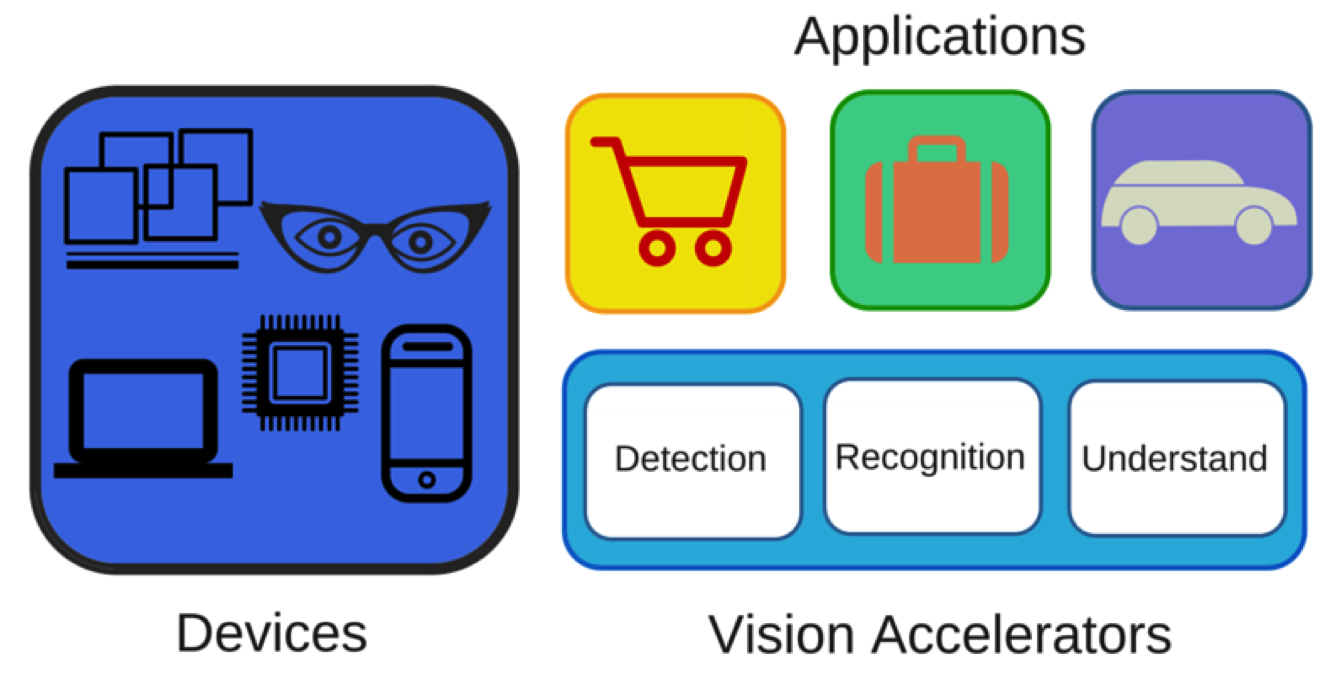
\includegraphics[width=0.9\linewidth]{./figures/vision_apps_devices.png}
\vspace{0pt}
\caption{Application-specific vision accelerator pipeline.}
\label{fig:iot}
\vspace{0pt}
\end{figure}

Fig.~\ref{fig:iot} illustrates the interaction between compute devices and vision accelerators when targeting various applications. A common vision pipeline involves parsing the visual scene and extracting objects or regions of interest (RoIs). This is 
carried out in the object detection stage. Once regions are extracted they are sent to a recognition stage to identify 
what the object is. Having figured out whether the object is of interest, further options can be explored. For example, if the 
object is a person, activity or pose estimation can be triggered. The application workload usually will decide the choice of 
the compute device. For example, if a user is in a retail store and would like to use a smart visual-assist device, a 
wearable small form-factor device would be ideal. However, if this is an automotive-assist system, a larger device may be 
engaged. If a security application is being deployed at an airport, then a large server-scale architecture would be needed to
handle the sheer volume of data being generated every minute.

The main contributions of this paper are:
\begin{itemize}
\item To usher in the next wave of technology, we explore the current state-of-the-art in 
embedded vision accelerators and lay emphasis on key insights when designing such accelerators.
\item With scaling technology paving the way for approximate computing, we exploit an increasingly powerful property of most vision algorithms - reliability to noise. 
We show that for an object recognition system using DRAMs for memory storage, we can reduce refresh rates by $4\times$ thus reducing refresh energy. We can also reduce the number of multipliers by $7\times$ in the preprocessing stage of the system. We maintain a 1\% error bound on accuracy while exploiting reliability of the system.
\end{itemize}

The rest of this paper is organized as follows:
In Section~\ref{sec:related}, we provide an overview of vision-based architectures and the corresponding state-of-the-art.
Section~\ref{sec:reliability} describes opportunities to optimize an object recognition application based on its error resilient capabilities.
Finally, we conclude with Section~\ref{sec:conclusion}.

% no \IEEEPARstart
%This demo file is intended to serve as a ``starter file''
%for IEEE conference papers produced under \LaTeX\ using
%IEEEtran.cls version 1.7 and later.
% You must have at least 2 lines in the paragraph with the drop letter
% (should never be an issue)
%I wish you the best of success.

%\hfill mds
 
%\hfill January 11, 2007

\section{Vision Accelerators}
\label{sec:related}

Due to the capacity of human vision systems for highly complex processing at very low power, many brain-inspired algorithms and architectures have been proposed to emulate the human visual cortex.~\cite{Nere2011,Chen2014,Kestur2012}. %[YiranChen UPitt, Qingriu Syracuse, NEC CNN]. 

%DSPs
Digital signal processors (DSPs) have been a universally accepted alternative to general purpose CPUs for seamless multimedia processing. 
The Qualcomm Hexagon DSP instruction set architecture (ISA) contains numerous special-purpose instructions designed to accelerate key multimedia kernels such as 
sliding window filtersi~\cite{hexagon}. Similarly, Texas Instruments has a heterogenous multi-core DSP targeted for real-time vision applications 
based on their Keystone architecture.

%Heterogenous Architectures
To tackle the diverse field of vision many other heterogenous architectures have been proposed that take advantage of 
customized flows for regular systolic operations while
using the traditional von Neumann architecture for handling control logic and other irregular data operations. A heterogenous server architecture consisting of 
many small cores for low power and high throughput coupled with custom hardware accelerators was designed in ~\cite{Iyer2011}.
In ~\cite{HPCA2015}, the authors explored architectural heterogeniety by using customized data-flows for many vision-based applications targeted at retail, 
security, etc.

%Custom Accelerators
Custom vision accelerators have shown to be extremely performance-friendly for computationaly intensive tasks such as face detecion ~\cite{violafccm}, pedestrian detection~\cite{sips2014}, object recognition~\cite{Maashri2012a} and object detection~\cite{Bae2011}.

%CNNs
Even though Convolutional Neural Networks (CNNs) were explored in the early 1990s for vision applications~\cite{giles1997}, they have resurfaced again after a long hiatus and become extremely popular in the past couple of years. 
This successful comeback can be attributed to two major phenomena:
(1) the existence of large amount of data (needed to train the network well) with the evolution of the digital era, and (2) the development of 
custom hardware (required for acceleration) now being used for CNNs. 

In the ImageNet Large Scale Visual Recognition Challenge (ILSVRC)
conducted in 2012, the winning team trained a CNN consisting of five convolutional and three fully-connected layers. Importantly, the depth of the CNN is critical to 
its recognition capabilities since the authors found that removing any convolutional layer resulted in inferior performance~\cite{NIPS2012}. This CNN would need
more than 80 million operations and over 100,000 data transfers~\cite{XilinxCNN}.

More recent and advanced CNN architectures have 10 to 20 layers of Rectified Linear Units, hundreds of millions of weights, and billions of connections between units.
The reader is pointed to ~\cite{Bengio2009} for insights on deep architectures in general and ~\cite{DNNNature2015} for CNN-based learning and their recent advances. 

From a systems perspective, ~\cite{Farabet2009} mapped an earlier Convolutional Network based face-detection task onto custom hardware. More recently, ~\cite{Chen2014} recently proposed an architecture for CNNs and Deep 
Neural Networks (DNNs) that minimized memory transfers thus achieving high
throughput with small area, power and energy footprint. ~\cite{DaDianNao} furthered this by proposing a training and inference accelerator 
capable of providing GPU-like bandwidth in ASIC-like power budgets.


\section{Leveraging Reliability in Vision}
\label{sec:reliability}
%Reliability
Reliability is being explored at different layers of abstraction; from devices~\cite{Datta2014,Datta2015,Rahul2015} to memory~\cite{isca2014} to algorithms.
At a circuit-level, ~\cite{chen2015fast} uses a conditional probability approach for modeling reliability in combinational circuits.

\subsection{Introduction}
In this section, we evaluate the capabilities of a popular visual object recognition algorithm - HMAX - and exploit the potential to save 
power and reduce computational load.

\subsection{HMAX}
HMAX is a hierarchical visual object recognition model that has been used in various embedded real-time applications~\cite{Kestur2012, Maashri2012a}. 

%HMAX Expt

\subsection{Exploiting Resiliency for Power Benefits}

So far we have surveyed the landscape of vision systems that enhance the 
performance and energy efficiency of the computational fabrics. 
However, memory is an integral part of most systems today and contributes 
between 10-30\% of the overall power of embedded video systems and 
mobile phones~\cite{CarrollAaronHeiser2010}. 
The increasing memory size in new generations of embedded systems and 
the use of stacked 3D architectures that increase on-chip temperatures 
have made researchers look at saving on memory refresh energy. 
New power-efficient techniques such as Low Power Auto Self Refresh, Temperature Controlled Refresh, Refresh Pausing, Fine Granularity Refresh and Data Bus 
Inversion have been introduced in new memory standards such as 
DDR4~\cite{jedec-sdram-standards}.  

Tuning DRAM refresh based on the data characteristics has been proposed as early as 1998~\cite{islped98}.  
Many recent works have looked at tackling the increasing refresh power in other 
different ways~\cite{Liu2012, Stuecheli2010}. In ~\cite{Liu2011}, the 
authors looked at reducing refresh power on multimedia workloads. Recently, in ~\cite{iccd2014}, the authors showed that in 
real-time embedded vision applications, refresh power can dynamically be changed based on autonomously tagging data with logical labels.

%HMAX Expt
\begin{figure*}[!htb]
\centering
\begin{tabular}{@{}c@{} @{}c@{}}
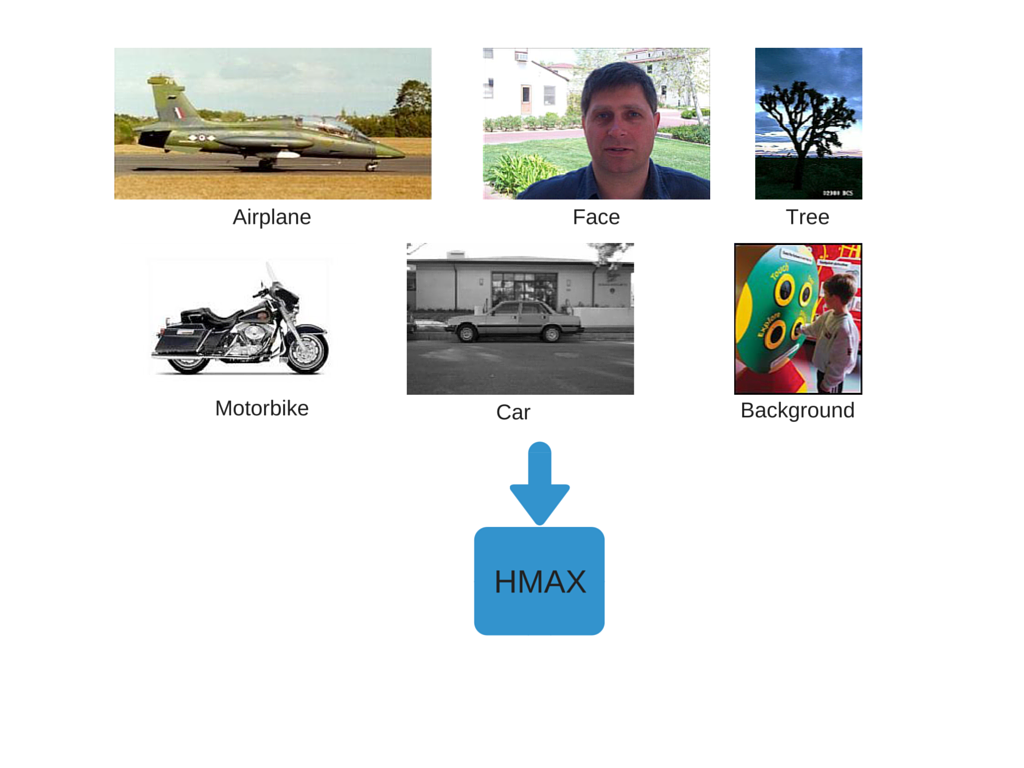
\includegraphics[width=0.45\linewidth]{./figures/hmax_reliability_a.png} & 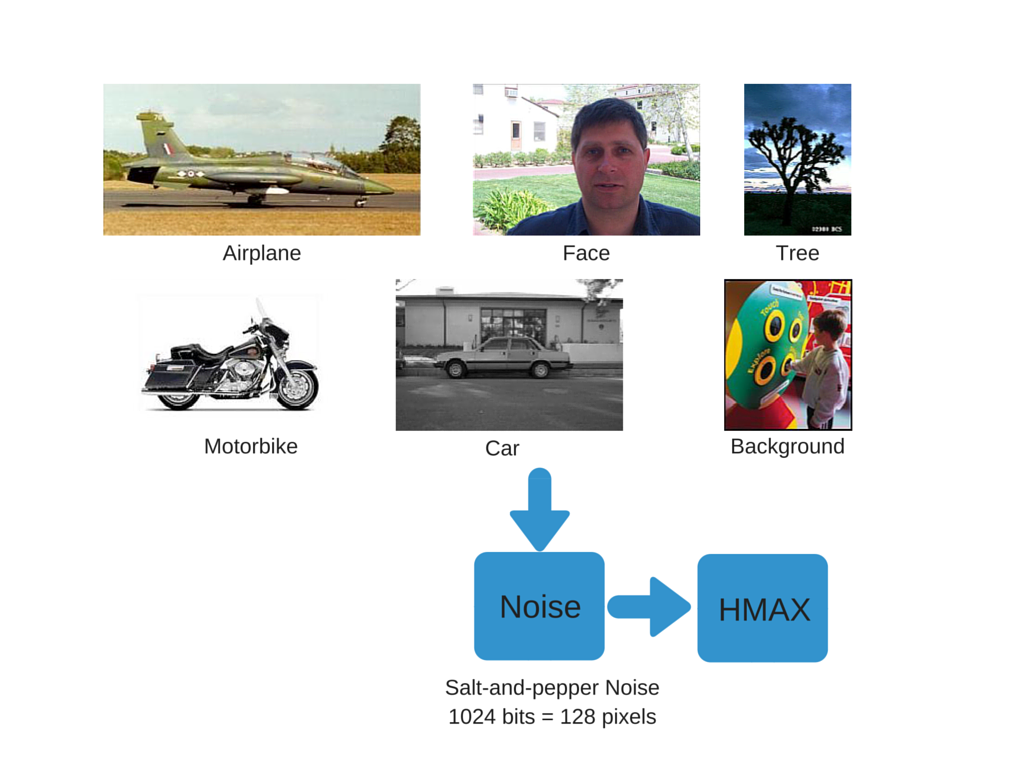
\includegraphics[width=0.45\linewidth]{./figures/hmax_reliability_b.png}\\[\abovecaptionskip]
\small (a) Baseline & \small (b) Noise
\end{tabular}
\vspace{1pt}
\caption{HMAX resilience to errors. Six classes from CalTech101 were used.}
\label{tab:hmax_reliability}
\end{figure*}

In this section, we explore the resiliency of HMAX to bit errors that can then be used to choose the refresh rate for DRAMs when these images are stored.  
Fig.~\ref{fig:hmax_pixel_sensitivity} illustrates the classification accuracy of HMAX as a function of the pixel errors introduced in each image.

%HMAX Resilience
\begin{figure}[htb!]
\vspace{0pt}
\centering
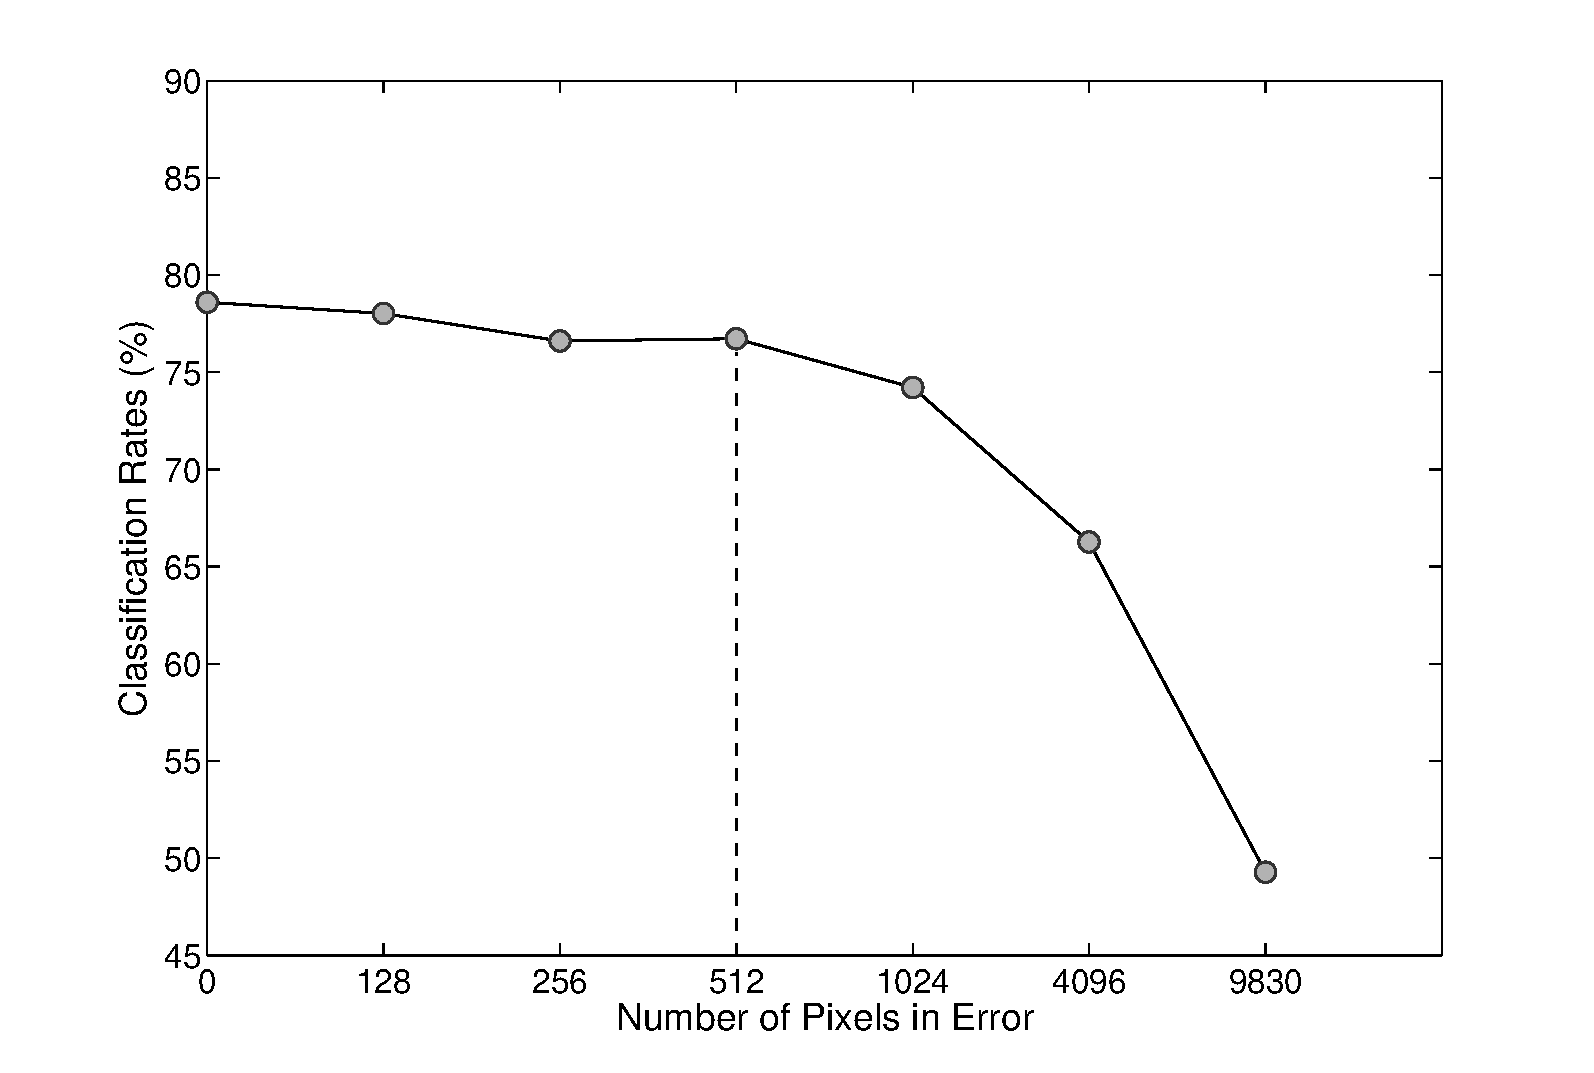
\includegraphics[width=0.99\linewidth,trim={20 20 30 20}, clip]{./figures/PixelSensitivityAnalysis.pdf}
\vspace{0pt}
\caption{HMAX resilience to errors. Six classes from CalTech101 were used.}\label{fig:hmax_pixel_sensitivity}
\vspace{0pt}
\end{figure}

\subsection{Exploiting Reseliency for Compute Benefits}
Image reconstruction is an important processing technique in image processing and computer vision applications. Most object recognition algorithms use a multi-scale 
pyramid to make it scale invariant. For example, HMAX uses an image pyramid having 11 scales (including base scale) with a scale factor of $2^{1/4}$ and 
uses a bicubic interpolation technique 
to generate the image pyramid. The input image is passed through this image pyramid before computing the ``S1'' layer of HMAX. 

%Interpolation
\begin{figure*}[!htb]
\centering
\begin{tabular}{@{}c@{} @{}c@{}}
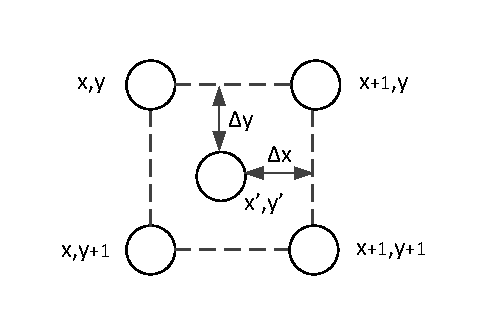
\includegraphics[width=0.3\textwidth]{./figures/bilinear.pdf} & 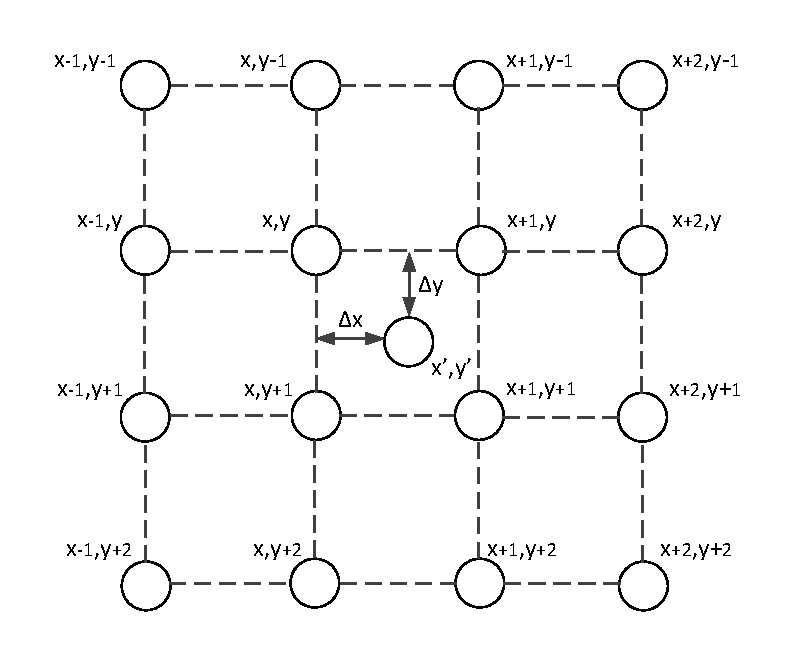
\includegraphics[width=0.5\textwidth]{./figures/bicubic.pdf}\\[\abovecaptionskip]
\small (a) Bilinear Interpolation & \small (b) Bicubic Interpolation
\end{tabular}
\vspace{1pt}
\caption{Interpolation techniques. In (a), four while in (b), 16 neighboring pixels are used for interpolation.}
\label{tab:interpolation}
\end{figure*}

Many architectures have been proposed to support linear 
and non-linear interpolation techniques~\cite{kesturdac}.

Given a pixel $I(x,y)$, an interpolated pixel $I'(x',y')$ using bilinear interpolation is given by ~(\ref{eq:1}). By definition, 
this involves computing two linear interpolation in $x$ and $y$ directions and requires eight multiplications. 
Figure~\ref{tab:interpolation}(a) illustrates an interpolated pixel using four neighboring pixels.

\begin{equation}
\begin{split}
I'(x',y') = &I(x,y) \times (1-\Delta x) \times (1-\Delta y) +\\ 
            &I(x+1,y) \times\Delta x \times (1-\Delta y) +\\ 
            &I(x,y+1) \times (1-\Delta x) \times\Delta y +\\ 
            &I(x+1,y+1) \times\Delta x \times\Delta y 
\end{split}
\label{eq:1}
\end{equation}

Using bicubic interpolation, the same interpolated pixel $I'(x',y')$ is given by ~(\ref{eq:2}) where 
$R_c$ denotes a bicubic interpolation function. The computation requires 56 multiplications in all and Figure~\ref{tab:interpolation}(b) shows the interpolated pixel 
using sixteen neighboring pixels.

\begin{equation}
\begin{split}
I'(x',y')=\sum_{m=-1}^{2}\sum_{n=-1}^{2}I(x+m,y+n)R_c(m-\Delta x)R_c(-(n-\Delta y))
\end{split}
\label{eq:2}
\end{equation}

In this section we explore the potential savings in computational work needed to be done while not compromising on accuracy. 
In the embedded version, compute resources are very costly. Saving a few resources can result in being able to 
fit a design in a particular form-factor or may cause the design to overflow into the next larger generation of devices. We explored the 
capablity of HMAX to correctly recognize objects using bilinear interpolation in the image pyramid. We used all 101 classes of CalTech101 
for this purpose. It should be noted that using the original bicubic interpolation technique, we achieve 54\% accuracy on the said dataset. This is in confirmation with the results shown in ~\cite{Mutch2008}. 
We then ran the experiment using bilinear interpolation and found the impact of this is a 1\% loss in accuracy. Also, instead of 
56 multipliers (bicubic interpolation), we would need just eight multipliers (bilinear interpolation). Table~\ref{table:compute} shows the 
results and the savings have a significant impact on area and performance of the accelerated system. 

\begin{table}[h]
\renewcommand{\arraystretch}{1.3}
\caption {Impact of Interpolation Techniques}
\label{table:compute}
\centering
\begin{tabular}{lllll}
 System & Algorithm & Accuracy & Multipliers\\\hline
 HMAX	& Bicubic   & 54\% & 56\\\hline
 HMAX   & Bilinear  & 53\% & 8\\\hline
\end{tabular}
\end{table}


% An example of a floating figure using the graphicx package.
% Note that \label must occur AFTER (or within) \caption.
% For figures, \caption should occur after the \includegraphics.
% Note that IEEEtran v1.7 and later has special internal code that
% is designed to preserve the operation of \label within \caption
% even when the captionsoff option is in effect. However, because
% of issues like this, it may be the safest practice to put all your
% \label just after \caption rather than within \caption{}.
%
% Reminder: the "draftcls" or "draftclsnofoot", not "draft", class
% option should be used if it is desired that the figures are to be
% displayed while in draft mode.
%
%\begin{figure}[!t]
%\centering
%\includegraphics[width=2.5in]{myfigure}
% where an .eps filename suffix will be assumed under latex, 
% and a .pdf suffix will be assumed for pdflatex; or what has been declared
% via \DeclareGraphicsExtensions.
%\caption{Simulation Results}
%\label{fig_sim}
%\end{figure}

% Note that IEEE typically puts floats only at the top, even when this
% results in a large percentage of a column being occupied by floats.


% An example of a double column floating figure using two subfigures.
% (The subfig.sty package must be loaded for this to work.)
% The subfigure \label commands are set within each subfloat command, the
% \label for the overall figure must come after \caption.
% \hfil must be used as a separator to get equal spacing.
% The subfigure.sty package works much the same way, except \subfigure is
% used instead of \subfloat.
%
%\begin{figure*}[!t]
%\centerline{\subfloat[Case I]\includegraphics[width=2.5in]{subfigcase1}%
%\label{fig_first_case}}
%\hfil
%\subfloat[Case II]{\includegraphics[width=2.5in]{subfigcase2}%
%\label{fig_second_case}}}
%\caption{Simulation results}
%\label{fig_sim}
%\end{figure*}
%
% Note that often IEEE papers with subfigures do not employ subfigure
% captions (using the optional argument to \subfloat), but instead will
% reference/describe all of them (a), (b), etc., within the main caption.


% An example of a floating table. Note that, for IEEE style tables, the 
% \caption command should come BEFORE the table. Table text will default to
% \footnotesize as IEEE normally uses this smaller font for tables.
% The \label must come after \caption as always.
%
%\begin{table}[!t]
%% increase table row spacing, adjust to taste
%\renewcommand{\arraystretch}{1.3}
% if using array.sty, it might be a good idea to tweak the value of
% \extrarowheight as needed to properly center the text within the cells
%\caption{An Example of a Table}
%\label{table_example}
%\centering
%% Some packages, such as MDW tools, offer better commands for making tables
%% than the plain LaTeX2e tabular which is used here.
%\begin{tabular}{|c||c|}
%\hline
%One & Two\\
%\hline
%Three & Four\\
%\hline
%\end{tabular}
%\end{table}


% Note that IEEE does not put floats in the very first column - or typically
% anywhere on the first page for that matter. Also, in-text middle ("here")
% positioning is not used. Most IEEE journals/conferences use top floats
% exclusively. Note that, LaTeX2e, unlike IEEE journals/conferences, places
% footnotes above bottom floats. This can be corrected via the \fnbelowfloat
% command of the stfloats package.

\section{Conclusion}
\label{sec:conclusion}
% Conclusion
In this paper we extensively survey a plethora of vision-based systems 
targeted for real-time applications. We also exploit the inherent robustness 
in vision algorithms and show that it can help to reduce both 
power and compute resources, both of which are valuable when designing systems.


% conference papers do not normally have an appendix


% use section* for acknowledgement
\section*{Acknowledgements}
\label{sec:acknowledgements}
%\section{Acknowledgements}
\label{sec:acknowledgements}
This work is supported in part by NSF Expeditions: Visual Cortex on Silicon CCF 1317560. The work is also supported through infrastructure provided by NSF Award 1205618.

%The authors would like to thank...

% trigger a \newpage just before the given reference
% number - used to balance the columns on the last page
% adjust value as needed - may need to be readjusted if
% the document is modified later
%\IEEEtriggeratref{8}
% The "triggered" command can be changed if desired:
%\IEEEtriggercmd{\enlargethispage{-5in}}

% references section

% can use a bibliography generated by BibTeX as a .bbl file
% BibTeX documentation can be easily obtained at:
% http://www.ctan.org/tex-archive/biblio/bibtex/contrib/doc/
% The IEEEtran BibTeX style support page is at:
% http://www.michaelshell.org/tex/ieeetran/bibtex/
%\bibliographystyle{IEEEtran}
% argument is your BibTeX string definitions and bibliography database(s)
%\bibliography{IEEEabrv,../bib/paper}
%
% <OR> manually copy in the resultant .bbl file
% set second argument of \begin to the number of references
% (used to reserve space for the reference number labels box)
%\begin{thebibliography}{1}

%\bibitem{IEEEhowto:kopka}
%H.~Kopka and P.~W. Daly, \emph{A Guide to \LaTeX}, 3rd~ed.\hskip 1em plus
%  0.5em minus 0.4em\relax Harlow, England: Addison-Wesley, 1999.

%\end{thebibliography}

\bibliographystyle{IEEEtran}
\small
\bibliography{IEEEabrv,library}


% that's all folks
\end{document}


